\documentclass[11pt,letterpaper]{article}

% --- Packages ---
\usepackage[margin=1in]{geometry}
\usepackage{graphicx}
\usepackage{amsmath}
\usepackage{booktabs} % For professional tables
\usepackage{cite}
\usepackage{titlesec}
\usepackage{abstract}
\usepackage{parskip}
\usepackage{subcaption}
\usepackage{multirow}
\usepackage{float}
\usepackage{hyperref}

% --- Document Formatting ---
\titleformat{\section}{\large\bfseries}{\thesection.}{0.5em}{}
\titleformat{\subsection}{\normalsize\bfseries}{\thesubsection.}{0.5em}{}
\titleformat{name=\section,numberless}{\large\bfseries}{}{0em}{}
\titleformat{name=\subsection,numberless}{\normalsize\bfseries}{}{0em}{}
\setlength{\parskip}{\baselineskip}

\title{\vspace{-1.5cm}\LARGE\bf Natural Disaster Tweets Classification Using Multimodal Data}
\author{
    Brian Zhang \\ Student ID: 1011197 \\
    \and
    Sabrina Wang \\ Student ID: 1011177 \\
    \and
    Sondre Kristiansen \\ Student ID: 1011228 \\
    \and
    Rasmus Tuokko \\ Student ID: 1011234 \\
}
\date{}

\begin{document}

\maketitle
\begin{center}
    \small\textit{Project repository:} \url{https://github.com/brian-w-zhang/Data-Science-Project}
\end{center}

\begin{abstract}
During natural disasters, social media carries critical but noisy signals for response teams. In this project, we build a binary classifier that predicts whether a post is disaster-informative or not using both text and image modalities. We combine the Kaggle ``NLP with Disaster Tweets'' dataset with CrisisMMD v2.0, applying class-balanced sampling across both sources to form the text branch training pool. Our PyTorch system uses a DistilBERT text branch, a ResNet50 vision branch with layer-wise freezing and differential learning rates, and a late-fusion MLP head that concatenates learned representations from both modalities. We apply learning rate scheduling and F1-based early stopping across all branches to improve convergence and mitigate overfitting. We compare unimodal and multimodal setups and report validation metrics from our training pipeline. We further implement a Streamlit chatbot-style interface that accepts tweet text and an optional image and returns a predicted label with confidence score. The project demonstrates that multimodal fusion is especially effective for emergency triage, where text and image may be individually ambiguous but jointly informative.
\end{abstract}

% ==========================================
\section{Introduction}
% ==========================================
%Define the machine learning problem you are investigating.
%\begin{itemize}
%    \item \textbf{Motivation:} Why is this an important problem? Frame this within the context of "AI for Security" or "AI for Social Good".
%    \item \textbf{Challenges:} Mention specific difficulties, such as extreme class imbalance (anomaly detection) or the complexity of fusing multiple modalities.
%    \item \textbf{Objectives:} State exactly what your model and UI are designed to achieve.
%\end{itemize}

This project investigates an automated binary classification problem: given the text and image of a tweet, determine whether it describes a real disaster or not. We train and evaluate models on a combination of two datasets: a text-only Kaggle disaster tweets dataset and a multimodal CrisisMMD dataset.

This problem lies at the intersection of AI for social good and AI for security. During natural and man-made disasters, people use Twitter to share real-time updates about injured or missing people, infrastructure damage, and urgent needs. If such crowd-sourced information can be filtered, classified, and surfaced quickly, it can support humanitarian organizations, emergency managers, and public safety agencies in gaining situational awareness and planning relief operations. At the same time, the ability to rapidly detect and assess emerging incidents from public sources contributes to broader security goals such as crisis detection, public warning, and resource deployment.

From a technical perspective, this setting presents several challenges. First, social media streams are noisy and ambiguous. Disaster-related words are often used metaphorically or jokingly, and many posts during a crisis are merely commentary rather than useful reports. Second, the CrisisMMD dataset exhibits class imbalance, with fewer non-disaster examples compared to disaster-related posts, which can bias the classifier.

The objectives of this work are based on the classification model and the user interface:
\begin{itemize}
    \item Develop and evaluate a multimodal machine learning model that classifies tweets as disaster and non-disaster, leveraging both text and images where available, and remaining robust to noisy, real-world data.
    \item Provide an interface where the user can write a tweet and immediately see how the model classifies it.
\end{itemize}

The remainder of this report is organized as follows. Section 2 reviews related work on disaster-related social media analysis, multimodal learning, and crisis informatics. Section 3 describes the datasets used in this study and how they were collected and combined, followed by Section 4, which details our preprocessing pipeline. Section 5 presents the proposed methodology and model architecture, and Section 6 outlines the experimental setup, including training procedures and evaluation metrics. Section 7 presents our results and performance visualizations. Section 8 describes the system implementation and the chatbot-style user interface. Finally, Section 9 concludes with a discussion of our findings, limitations, and directions for future work.

% ==========================================
\section{Related Work}
% ==========================================
The classification of disaster-related social media posts has evolved since the introduction of the CrisisMMD dataset by Alam et al. ($2018$)\cite{alam2018} They provided a benchmark for multi-modal humanitarian data. However, recent advancements have demonstrated the superiority of transformer-based architectures. In $2022$, a study came out using state of the art architectures in language models and image classification, combined on the CrisisMMD dataset.\cite{kotha2022} A couple different models were used and compared. Their findings conclusively demonstrated that multimodal late-fusion architectures outperform unimodal approaches when classifying disaster information.

\begin{table*}[h]
\centering
\caption{Accuracy (\%) for Informative vs Non-Informative using Text + Image Modality (Kotha et al., 2022)}
\label{tab:informative_fusion_results}

\resizebox{\textwidth}{!}{%
\begin{tabular}{@{}lccccc@{}}
\toprule
\textbf{Metric} & \textbf{Bert + VGG16} & \textbf{Bert + VGG19} & \textbf{Bert + ResNet50} & \textbf{Bert + Dense121} & \textbf{Bert + RegNetY320} \\ \midrule
Train Accuracy      & 99.94 & 99.96 & 100.0 & 100.0 & 100.0 \\
Validation Accuracy & 86.01 & 86.52 & 89.06 & 88.55 & 89.63 \\
Test Accuracy       & 86.50 & 86.83 & 88.00 & 89.50 & 89.63 \\
Precision           & 86.50 & 86.83 & 88.00 & 89.50 & 89.63 \\
Recall              & 86.50 & 86.83 & 88.00 & 89.50 & 89.63 \\
F1 Score            & 86.50 & 86.83 & 88.00 & 89.50 & 89.63 \\ \bottomrule
\end{tabular}%
} % --- End of resizebox ---

\end{table*}

% ==========================================
\section{Dataset Collection and Sources}
% ==========================================
To enrich the training data for our text branch, we draw samples from two publicly available sources: the Kaggle ``Natural Language Processing with Disaster Tweets'' dataset \cite{kaggle_dataset}, which contains over $10,000$ manually classified tweets, and the \textbf{CrisisMMD (v2.0)} dataset \cite{alam2018}, a publicly available repository containing over $16,000$ multimodal social media posts collected during seven major natural disasters in $2017$. From each source, up to $5,000$ examples per class are sampled before concatenation, ensuring neither source dominates the training distribution.

For vision and fusion training, we utilize CrisisMMD exclusively, as it is the only source with paired images. The objective of our machine is to classify posts as \textit{Informative}, indicating a real disaster requiring humanitarian aid, or \textit{Not Informative} (safe).

A core challenge in analyzing social media data is modality dissonance - for example, a user might post a devastating image of a collapsed bridge along an uninformative text caption. To prevent our model from filtering out critical visual evidence due to poor text descriptions, a tweet gets flagged if the image \textbf{or} the text is \textit{Informative}:
\[
\text{label} = 1 \iff \text{text\_info} = \textit{informative} \;\mathbf{OR}\; \text{image\_info} = \textit{informative}
\]

% ==========================================
\section{Data Pre-processing}
% ==========================================
The CrisisMMD dataset contain extraneous metadata and multi-task annotations. For instance, annotations include secondary labels \textit{Humanitarian Categories} and \textit{Damage Severity Assessment}. To strictly optimize our architecture for rapid binary emergency triage, we stripped the dataframe of these secondary labels columns prior to training. This dimensionality reduction not only prevents the models from relying on potentially noisy or absent metadata, but also significantly reduces the overall computational need.

\subsection{Text Pre-processing}
Raw Twitter text is highly unstructured and filled with artifacts that degrade the performance of language models. To ensure the DistilBERT \cite{distilbert} model focused purely on semantic emergency context, we implemented a strict Regular Expression (RegEx) pipeline in \texttt{data/text\_cleaner.py}, applied consistently at data load time for both training and inference. First, we removed all URLs and user mentions (@username), as these act as disruptive noise and could cause the model to overfit to specifics. Secondly, we addressed the problem of emojis and non-ASCII Unicode characters (e.g, \textit{â, €, ™}), since these cause encoding errors and thus impact the performance. The cleaned text was then padded and truncated to a standardized maximum length of $128$ tokens.

\subsection{Image Pre-processing}
To process the visual data, we utilized a standard computer vision pipeline via \textit{torchvision} to prepare the images for the ResNet50 \cite{resnet50} feature extractor. Images were resized and center-cropped to $224\times224$ pixels to satisfy the architectural requirements of the ResNet model. The pixel values were subsequently normalized using ImageNet standard means $[0.485, 0.456, 0.406]$ and standard deviations $[0.229, 0.224, 0.225]$ to ensure optimal gradient convergence during training.

We apply separate transform pipelines for training and evaluation. Training transforms include random augmentation (random horizontal flips ($p=0.5$), rotations up to $15°$, and color jitter (brightness $\pm 0.2$)) to reduce overfitting to specific image appearances. Evaluation transforms apply only deterministic resizing and cropping, ensuring consistent results at inference time. Images are loaded in RGB; palette (RGBA) images are composited onto a white background prior to conversion, preventing color corruption from naive alpha-channel dropping.

\subsection{Handling Class Imbalance of CrisisMMD}
A significant challenge inherent to the CrisisMMD dataset is the severe class imbalance. In our processed dataset, the distribution is highly skewed: $13,784$ posts (approximately 76\%) are classified as \textit{Informative} (Disaster), while only $4,298$ posts (24\%) are \textit{Not Informative} (Safe).

If we leave it unaddressed, this imbalance leads to the ``accuracy paradox'' during neural network training. A naive model can achieve an accuracy of 76\% simply by predicting the majority class for every single input. Consequently, the model would fail entirely at its primary task.

A common preliminary approach to severe imbalance is random undersampling, deleting thousands of majority class instances to achieve a 50/50 split. This method is highly detrimental here, since deep architectures like DistilBERT and ResNet50 are dependent on huge data. Deleting nearly $9,500$ \textit{Informative} tweets would artificially starve the networks, and ignore diverse examples of real-world emergencies. This massive loss of variance would cause the models to severely overfit to the remaining small dataset. Instead, we address imbalance through weighted cross-entropy loss, computing per-class weights from the training label distribution: $w_\text{safe} = 4.207$, $w_\text{disaster} = 1.312$.

% ==========================================
\section{Methodology and Architecture}
% ==========================================

\subsection{Baseline Models}
To contextualize the performance of the final multimodal model, we evaluate against three reference configurations. The first is a naive majority classifier that always predicts the dominant class, yielding $70.92\%$ accuracy on the CrisisMMD benchmark and serving as a lower bound that quantifies the effect of class skew. The second is a DistilBERT model fine-tuned solely on tweet text, which achieves $86.29\%$ accuracy on the combined Kaggle and CrisisMMD text corpus, a $15.37$ percentage point improvement over the majority baseline and an indication that textual cues alone carry strong discriminative signal. The third is a ResNet50 model fine-tuned solely on CrisisMMD images. Together, these unimodal baselines allow us to assess whether multimodal fusion provides genuine complementary gains or simply inherits the performance of the stronger individual branch.

\subsection{Proposed Multi-Modal Architecture}
The multi-modal architecture comprises a text branch, a vision branch, and a late fusion model. All models are implemented in PyTorch using reusable classes and functions for data loading, training, and evaluation.

For the text branch, we use DistilBERT (\texttt{distilbert-base-uncased}) to encode tweet text. Input text is tokenized with a maximum sequence length of $128$ and passed through a sequence-classification setup, producing a $768$-dimensional [CLS] token representation that captures the overall semantic context of the tweet.

For the vision branch, we use ResNet50 pretrained on ImageNet \cite{imagenet} as the image encoder. To preserve the low-level texture and edge features learned during ImageNet pre-training while allowing the higher-level layers to adapt to disaster imagery, we apply a layer-wise freezing strategy: the first two residual blocks (\texttt{layer1}, \texttt{layer2}) are kept frozen throughout, while \texttt{layer3}, \texttt{layer4}, and the final fully-connected layer are unfrozen and trained with differential learning rates. This graduated approach reflects the conventional understanding that early ResNet layers encode generic visual features (edges, textures) that transfer broadly across domains, while later layers encode task-specific high-level patterns that benefit from domain adaptation. The ResNet50 encoder produces a $2048$-dimensional feature vector.

The fusion model concatenates the DistilBERT and ResNet50 representations into a single $2816$-dimensional vector, which is passed through a trainable MLP classifier head:

\[
2816 \rightarrow 512 \xrightarrow{\text{ReLU + Dropout}(0.5)} 2.
\]

During fusion training, the text and vision encoders are kept frozen so that only the MLP classifier head is optimized. This prevents catastrophic forgetting of the pretrained representations and keeps fusion training computationally tractable, while the fixed encoder outputs serve as rich multimodal embeddings for the learned fusion stage.

% ==========================================
\section{Experimental Setup}
% ==========================================

\subsection{Training Strategy}
All branches use an $80/20$ train/validation split with a fixed random seed applied to Python, NumPy, and PyTorch random number generators for full reproducibility. Checkpoints are saved to Google Drive during training, with each branch persisting its best weights whenever validation macro F1 improves.

The choice of macro F1 as the checkpoint selection criterion is central to our training strategy. Under class imbalance, validation loss can decrease monotonically even as the model progressively neglects the minority class. A model that hedges toward the dominant disaster class achieves lower cross-entropy while failing entirely on non-informative tweets. By tracking macro F1, which weights each class equally, we ensure that the retained checkpoint corresponds to the most balanced classifier across training, rather than the one that happens to minimize cross-entropy at a given epoch.

\subsection{Hyperparameter Tuning}
Initial training runs revealed signs of overfitting in the vision branch, with training loss decreasing steadily while validation loss reversed and trended upward after the first few epochs. To counter this, we introduced several targeted adjustments.

Differential learning rates are applied across ResNet50's unfrozen layers: \texttt{layer3} is trained at $1\times10^{-5}$, \texttt{layer4} at $1\times10^{-4}$, and the final fully-connected layer at $1\times10^{-3}$. This graduated schedule allows the task-specific higher-level layers to adapt more aggressively while protecting the general low-level features retained from ImageNet pre-training. A StepLR scheduler decays all rates by a factor of $0.5$ every three epochs, preventing the optimizer from overshooting in later training stages. Training-time augmentation, including random horizontal flips ($p=0.5$), rotations up to $15°$, and color jitter (brightness $\pm0.2$), further reduces overfitting to specific image appearances by increasing the effective diversity of the training distribution.

For the text branch, we use the AdamW optimizer at a learning rate of $1\times10^{-5}$ with a cosine warmup scheduler over the first $10\%$ of total training steps. The warmup is especially important for fine-tuning pre-trained transformers, as large initial update steps can disrupt the pretrained weights before the model has established a coherent gradient direction for the new task. The warmup linearly increases the learning rate from near zero to the target rate, followed by a cosine decay, allowing DistilBERT to gently transition from its pre-trained state toward the disaster classification objective. Maximum training is $10$ epochs with early stopping patience of $3$ and batch size $16$.

For the vision branch, the Adam optimizer is configured with the differential learning rates described above, CrossEntropyLoss, and batch size $32$, with a maximum of $15$ epochs and early stopping patience of $3$.

For the fusion head, Adam is applied to the MLP parameters only at a learning rate of $1\times10^{-3}$, with weighted CrossEntropyLoss using class weights $[w_\text{safe}=4.207,\ w_\text{disaster}=1.312]$ computed from the training label distribution. A ReduceLROnPlateau scheduler halves the learning rate when validation macro F1 stagnates for two consecutive epochs. The MLP uses $0.5$ dropout, batch size $32$, maximum $20$ epochs, and early stopping patience of $4$.

\subsection{Evaluation Metrics}
We report validation accuracy, binary and macro F1-score, ROC-AUC, and confusion matrices. Accuracy alone is an unreliable indicator on this imbalanced dataset, as a majority-class predictor achieves $70.92\%$ accuracy while failing entirely on non-informative tweets. Macro F1 weights both classes equally and directly captures the ability to distinguish informative from non-informative posts. ROC-AUC measures discriminative ability across all classification thresholds, independent of any specific operating point. Confusion matrices provide a granular breakdown of false negatives, i.e., disaster tweets incorrectly classified as safe, and false positives, which is especially informative in emergency triage contexts where failing to surface a genuine disaster signal has high real-world cost.
% ==========================================
\section{Results and Discussion}
% ==========================================

\subsection{Initial Training Results}
Training and validation curves, confusion matrices, and ROC curves from the initial training runs for all three branches are presented below. In these initial runs, checkpoint selection for the text branch was based on minimum validation loss rather than macro F1, and comprehensive per-class evaluation metrics were not yet tracked across all branches. These figures serve as the baseline against which the pipeline refinements introduced in Section 7.2 are compared. To recreate these figures from saved checkpoints without retraining, run only the setup cells and the ``Evaluation on best checkpoint'' section of each notebook (01\_text\_branch\_train.ipynb, 02\_vision\_branch\_train.ipynb, 03\_fusion\_layer\_train.ipynb). See Section~8.2 for full instructions.

\subsubsection{Text branch}

\begin{figure}[H]
    \centering
    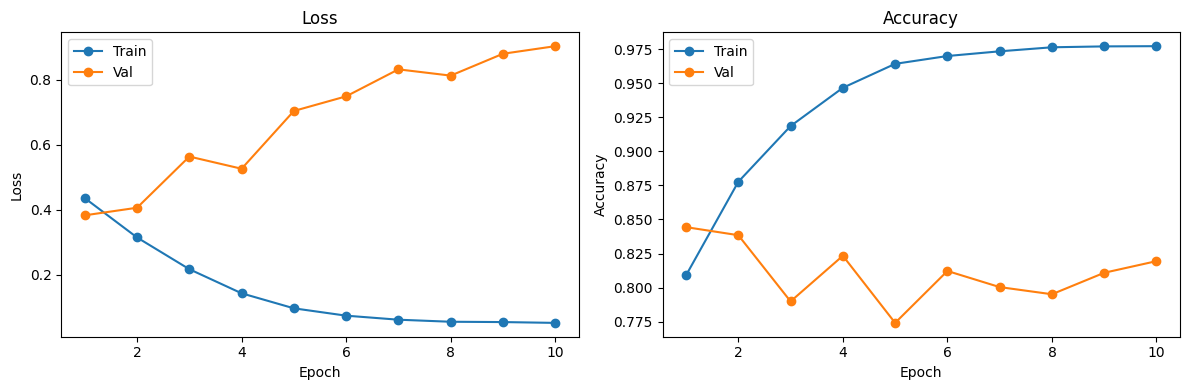
\includegraphics[width=1.0\linewidth]{kaggle-train.png}
    \caption{Training and validation loss/accuracy curves for the DistilBERT text branch (initial run). The model converges rapidly; the best checkpoint was selected at epoch 1 based on minimum validation loss.}
    \label{fig:kaggle_train}
\end{figure}

\begin{figure}[H]
    \begin{subfigure}{0.54\textwidth}
        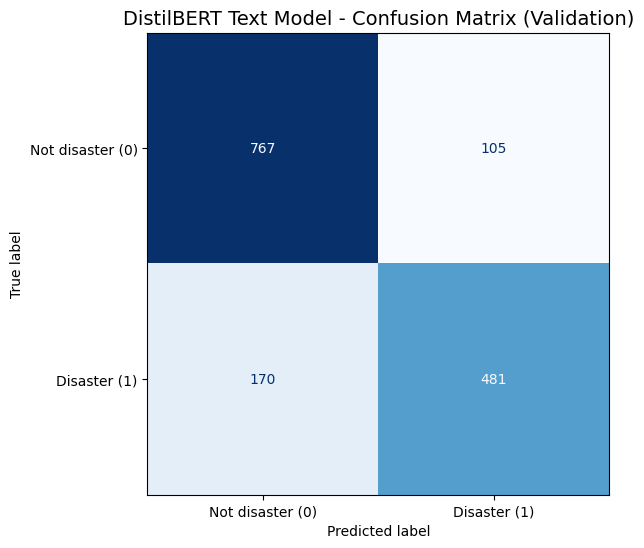
\includegraphics[width=0.9\linewidth]{kaggle-confmat.png}
        \caption{Confusion matrix on the validation set.}
        \label{fig:kaggle_confmat}
    \end{subfigure}
    \begin{subfigure}{0.46\textwidth}
        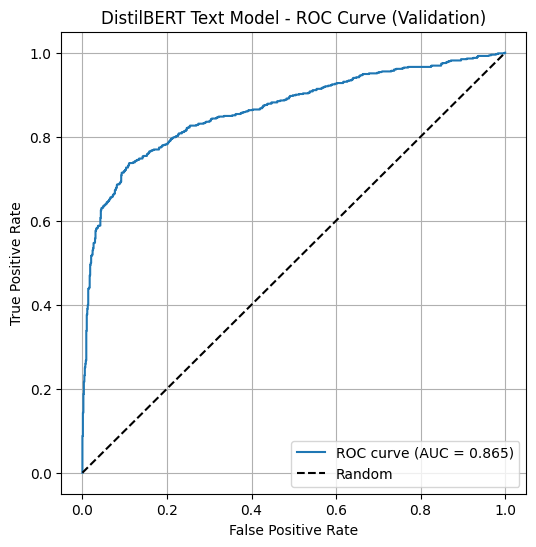
\includegraphics[width=0.9\linewidth]{kaggle-roc.png}
        \caption{ROC curve on the validation set.}
        \label{fig:kaggle_roc}
    \end{subfigure}
    \caption{Initial validation results for the DistilBERT text branch. The misclassifications lean toward false negatives.}
\end{figure}

The training curves in Figure \ref{fig:kaggle_train} show that the DistilBERT text model converges very quickly: training loss continue to decrease and training accuracy approaches 0.92, while the validation curves flatten and begin to diverge after the first epoch, indicating the onset of overfitting. Minimum validation loss is achieved at epoch 1 and thus selected as the checkpoint. The confusion matrix in Figure \ref{fig:kaggle_confmat} indicates a moderate skew toward false negatives: 170 disaster tweets are misclassified as non-disaster, compared to 105 false positives, which means the text-only model sacrifices some recall on true disasters. The ROC curve in Figure \ref{fig:kaggle_roc} (AUC $\approx$ 0.87) nevertheless indicates that the model ranks disaster vs. non-disaster tweets reasonably well, but the operating threshold implied by the default argmax is conservative for the positive class.

\subsubsection{Vision branch}

\begin{figure}[H]
    \centering
    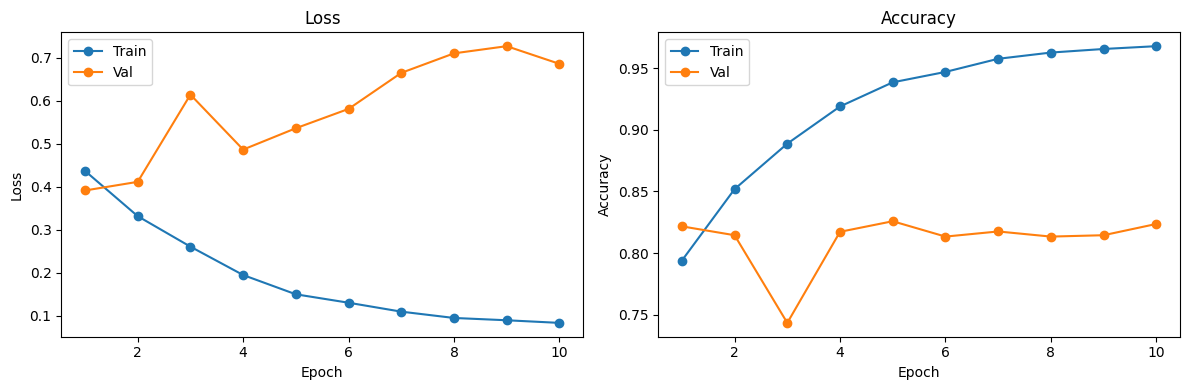
\includegraphics[width=1\linewidth]{resnet-train.png}
    \caption{Training and validation loss/accuracy curves for the ResNet50 vision branch. The model with minimal loss at epoch 1 was selected as the checkpoint.}
    \label{fig:resnet_train}
\end{figure}

\begin{figure}[H]
    \begin{subfigure}{0.53\textwidth}
        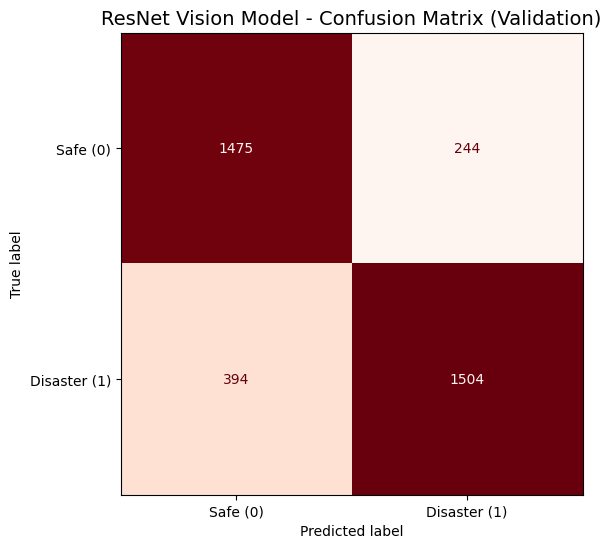
\includegraphics[width=0.9\linewidth]{resnet-confmat.png}
        \caption{Confusion matrix on the validation set.}
        \label{fig:resnet_confmat}
    \end{subfigure}
    \begin{subfigure}{0.47\textwidth}
        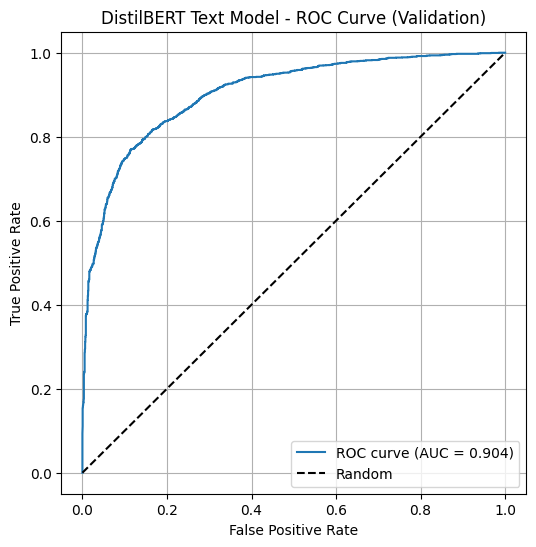
\includegraphics[width=0.9\linewidth]{resnet-roc.png}
        \caption{ROC curve on the validation set.}
        \label{fig:resnet_roc}
    \end{subfigure}
    \caption{Initial validation results for the ResNet50 vision branch. The misclassifications lean toward false negatives.}
\end{figure}

For the vision branch, the training curves in Figure \ref{fig:resnet_train} show a steeper improvement on the training set than on the validation set. Training accuracy climbs toward 0.97 and loss drops steadily, whereas validation accuracy oscillates around the low 0.80 range. The validation loss increases after the first epoch, again suggesting overfitting beyond the initial epochs. The confusion matrix in Figure \ref{fig:resnet_confmat} highlights a pattern similar to the text model, with more false negatives than false positives. However, the true-positive count remains high, and the ROC curve in Figure \ref{fig:resnet_roc} (AUC $\approx$ 0.90) indicates that the visual features are informative for distinguishing disaster from non-disaster imagery even if the chosen threshold leads to missed disasters.

\subsubsection{Fusion model}

\begin{figure}[H]
    \centering
    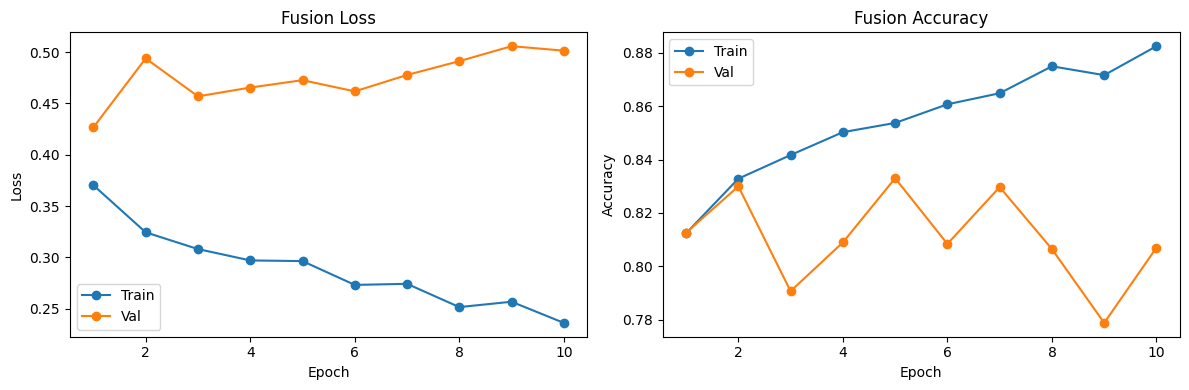
\includegraphics[width=1\linewidth]{fusion-train.png}
    \caption{Training and validation loss/accuracy curves for the late-fusion MLP head. Only the fusion classifier is trained; the frozen encoders supply fixed representations.}
    \label{fig:fusion_train}
\end{figure}

\begin{figure}[H]
    \begin{subfigure}{0.53\textwidth}
        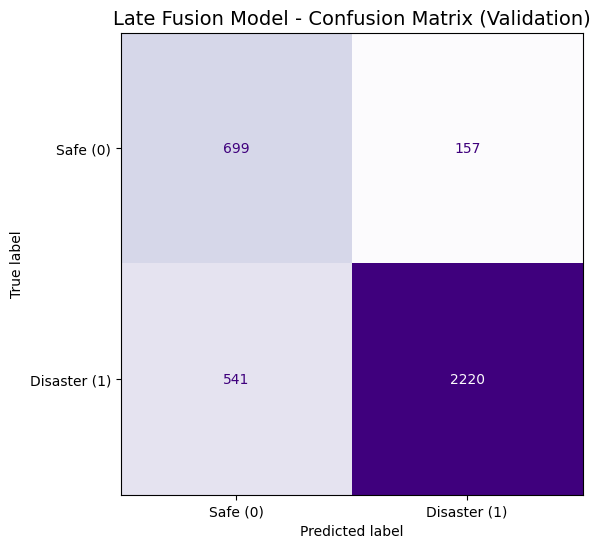
\includegraphics[width=0.9\linewidth]{fusion-confmat.png}
        \caption{Confusion matrix on the validation set.}
        \label{fig:fusion_confmat}
    \end{subfigure}
    \begin{subfigure}{0.47\textwidth}
        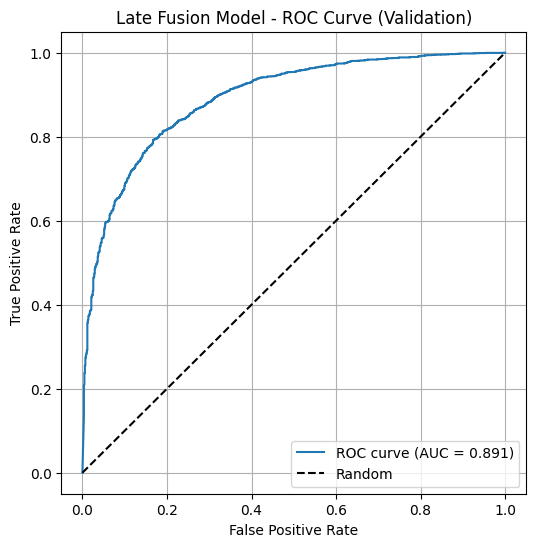
\includegraphics[width=0.9\linewidth]{fusion-roc.png}
        \caption{ROC curve on the validation set.}
        \label{fig:fusion_roc}
    \end{subfigure}
    \caption{Initial validation results for the fusion model. The misclassifications heavily lean toward false negatives.}
\end{figure}

The late-fusion training curves in Figure \ref{fig:fusion_train} show that while the fusion head learns steadily on the training set, the validation loss remains substantially higher. The validation accuracy fluctuates without a clear upward trend, pointing to limited generalization and some overfitting of the small MLP on top of the frozen encoders. Compared to the unimodal branches, the confusion matrix in Figure \ref{fig:fusion_confmat} is more polarized: the model correctly identifies a large number of disasters (2,200 true positives) but still produces substantially more false negatives than false positives, suggesting a bias toward predicting the negative class when modalities disagree or evidence is weak. The ROC curve in Figure \ref{fig:fusion_roc} (AUC $\approx$ 0.89) is stronger than the text branch and comparable to the vision branch. Recall of disasters remains a concern in the final fusion step.

\subsection{Training Pipeline Refinements}

Examining the initial results revealed two interconnected limitations in the training pipeline that warranted targeted correction.

The first was the choice of checkpoint selection criterion for the text branch. In the initial run, the best model weights were saved at the epoch with minimum validation loss, which turned out to be epoch 1, the same point at which the model has barely departed from its pretrained initialization. Under class imbalance, validation loss and macro F1 do not necessarily improve in tandem: a model can reduce cross-entropy loss by shifting its predictions toward the majority disaster class without meaningfully improving recall on the minority safe class. The initial text branch binary F1 of $0.7777$ reflects exactly this dynamic, as the model's safe-class recall was underdeveloped relative to its disaster-class performance. Applying F1-macro early stopping across all three branches ensures that the retained checkpoint corresponds to the most balanced classifier seen during training, directly penalizing failure on either class rather than optimizing for an aggregate loss that can be gamed by majority-class hedging.

The second limitation was the absence of a learning rate warmup for the text branch. Pre-trained transformer models like DistilBERT encode rich linguistic representations in their weight matrices. When fine-tuning begins with a full-magnitude learning rate, the relatively large gradient updates in the first few steps can disrupt these representations before the model has established a coherent gradient direction suited to the new task. This issue is particularly acute in the early epochs, where the randomly initialized classification head generates high-loss outputs that propagate large and potentially destabilizing gradient signals into the frozen-but-sensitive transformer layers. A cosine warmup scheduler addresses this by linearly increasing the learning rate from near zero to the target value over the first $10\%$ of training steps, then decaying it following a cosine curve for the remainder. This warm start allows DistilBERT to gently adjust from its pretrained state toward the disaster classification objective before committing to a direction in the parameter landscape.

These two changes are complementary. The warmup ensures that early training epochs produce meaningful and stable improvements in F1 rather than noisy fluctuations driven by large gradient steps, while the F1-based checkpoint criterion ensures that whichever epoch achieves the best balance between precision and recall is the one ultimately evaluated. Together, they allow the text branch to train productively beyond epoch 1 and reach a checkpoint with better minority-class recovery.

\subsection{Refined Training Results}

After applying the pipeline refinements, we re-ran all three branches and collected full per-class evaluation metrics, confusion matrices, and ROC curves.

\subsubsection{Text branch}

\begin{figure}[H]
    \centering
    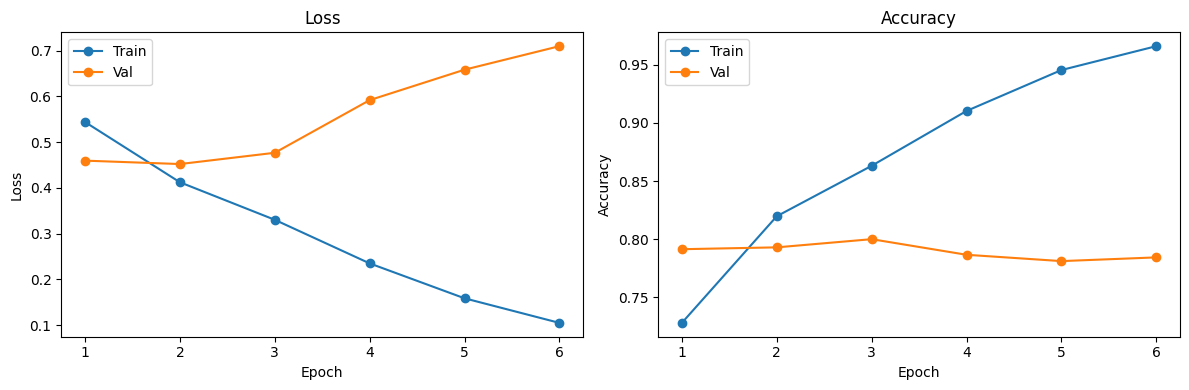
\includegraphics[width=1.0\linewidth]{nb01_img00.png}
    \caption{Training and validation loss/accuracy curves for the DistilBERT text branch (refined run). With cosine warmup and F1-macro early stopping, the best checkpoint is selected at epoch 3 rather than epoch 1.}
    \label{fig:kaggle_train_new}
\end{figure}

\begin{figure}[H]
    \begin{subfigure}{0.54\textwidth}
        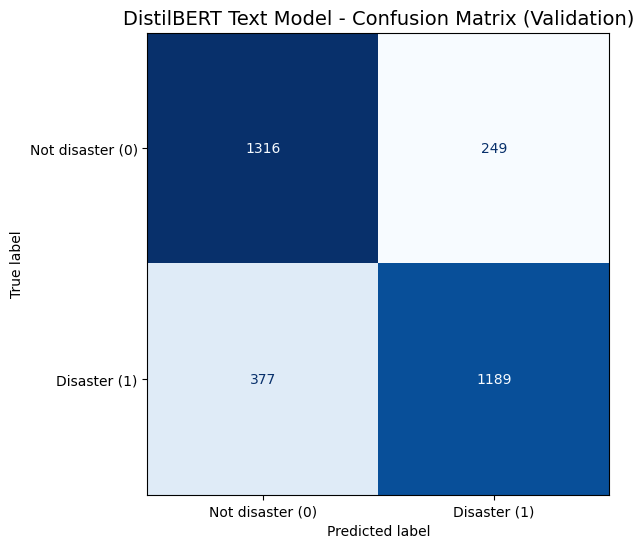
\includegraphics[width=0.9\linewidth]{nb01_img01.png}
        \caption{Confusion matrix on the validation set.}
        \label{fig:kaggle_confmat_new}
    \end{subfigure}
    \begin{subfigure}{0.46\textwidth}
        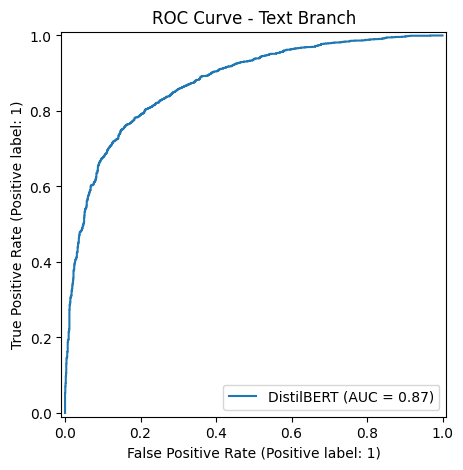
\includegraphics[width=0.9\linewidth]{nb01_img02.png}
        \caption{ROC curve on the validation set.}
        \label{fig:kaggle_roc_new}
    \end{subfigure}
    \caption{Refined text branch evaluation results. The best checkpoint at epoch 3 achieves $80.01\%$ accuracy, macro F1 of $0.7997$, and ROC-AUC of $0.8749$.}
    \label{fig:kaggle_eval_new}
\end{figure}

The F1-based early stopping selected epoch 3 as the best checkpoint, compared to epoch 1 in the initial run. The training curve shows that with the cosine warmup in place, validation macro F1 improves steadily through the first three epochs ($0.7910 \to 0.7924 \to 0.7997$) before the model begins to overfit in epochs 4 through 6, at which point the patience counter triggers and training halts. The confusion matrix reflects the improved minority-class recovery: false negatives decreased and the model's predictions are more balanced across classes than the initial run. Macro F1 improved to $0.7997$ and ROC-AUC to $0.8749$, both above the initial values. Notably, raw accuracy decreased marginally from $81.94\%$ to $80.01\%$: this is the expected trade-off when optimizing for macro F1 rather than accuracy, as the model makes fewer easy majority-class predictions and more genuine minority-class recoveries.

\subsubsection{Vision branch}

\begin{figure}[H]
    \centering
    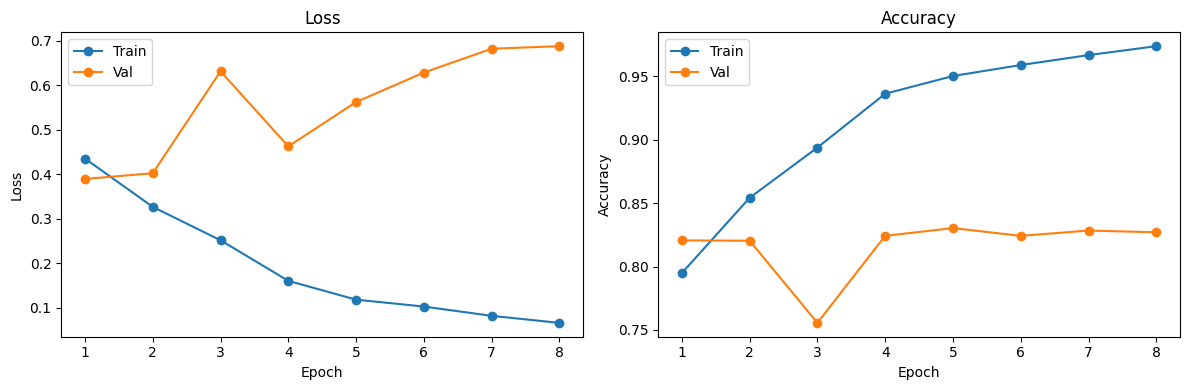
\includegraphics[width=1\linewidth]{nb02_img00.png}
    \caption{Training and validation loss/accuracy curves for the ResNet50 vision branch (refined run). The best checkpoint is selected at epoch 5 based on macro F1.}
    \label{fig:resnet_train_new}
\end{figure}

\begin{figure}[H]
    \begin{subfigure}{0.53\textwidth}
        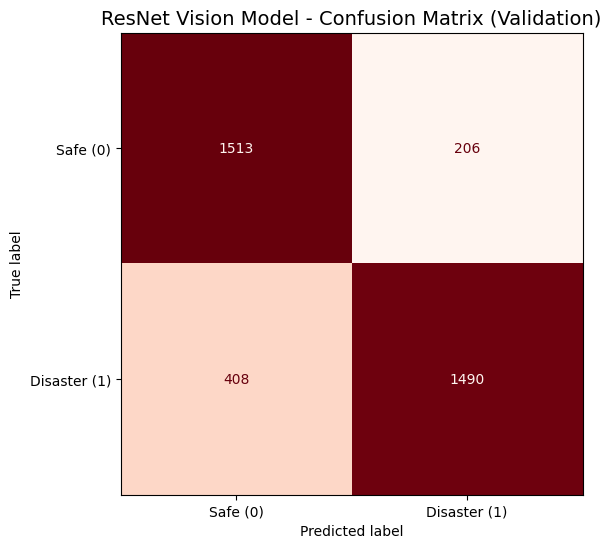
\includegraphics[width=0.9\linewidth]{nb02_img01.png}
        \caption{Confusion matrix on the validation set.}
        \label{fig:resnet_confmat_new}
    \end{subfigure}
    \begin{subfigure}{0.47\textwidth}
        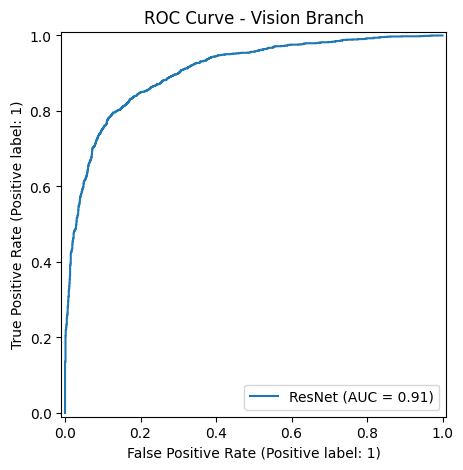
\includegraphics[width=0.9\linewidth]{nb02_img02.png}
        \caption{ROC curve on the validation set.}
        \label{fig:resnet_roc_new}
    \end{subfigure}
    \caption{Refined vision branch evaluation results. The best checkpoint achieves $83.02\%$ accuracy, macro F1 of $0.8302$, and ROC-AUC of $0.9059$.}
    \label{fig:resnet_eval_new}
\end{figure}

The vision branch, which already incorporated differential learning rates and StepLR scheduling from the initial runs, showed the most stable training behavior of the three branches. The validation accuracy curve exhibits a characteristic dip at epoch 3, a transient instability where the StepLR decay coincides with a particularly challenging batch distribution, before recovering and stabilizing around $83\%$ for the remainder of training. With F1-macro early stopping, the selected checkpoint at epoch 5 achieves $83.02\%$ accuracy, macro F1 of $0.8302$, and ROC-AUC of $0.9059$, representing modest but consistent improvements over the initial run. The classification report shows balanced precision and recall for both classes: precision $0.79$ and recall $0.88$ for the safe class, and precision $0.88$ and recall $0.79$ for the disaster class.

\subsubsection{Fusion model}

\begin{figure}[H]
    \centering
    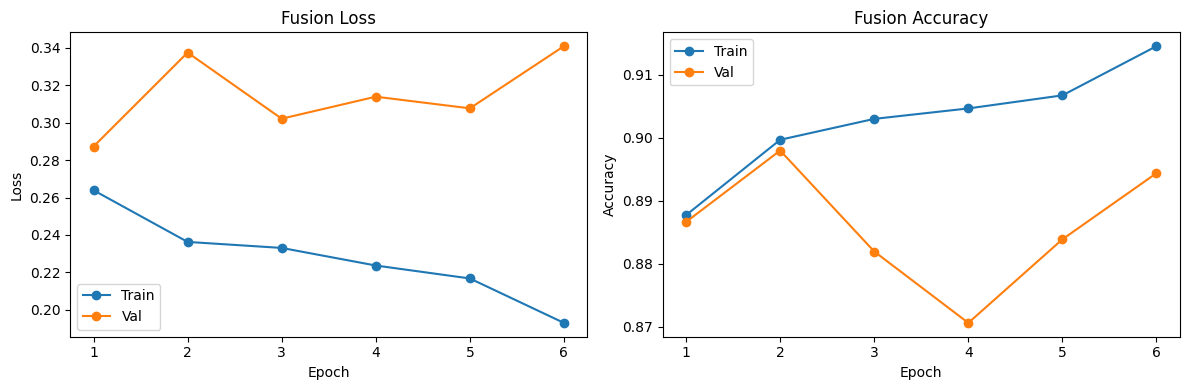
\includegraphics[width=1\linewidth]{nb03_img00.png}
    \caption{Training and validation loss/accuracy curves for the late-fusion MLP head (refined run). Validation accuracy reaches its peak at epoch 2 and degrades mildly thereafter as the head begins to overfit the fixed encoder representations.}
    \label{fig:fusion_train_new}
\end{figure}

\begin{figure}[H]
    \begin{subfigure}{0.53\textwidth}
        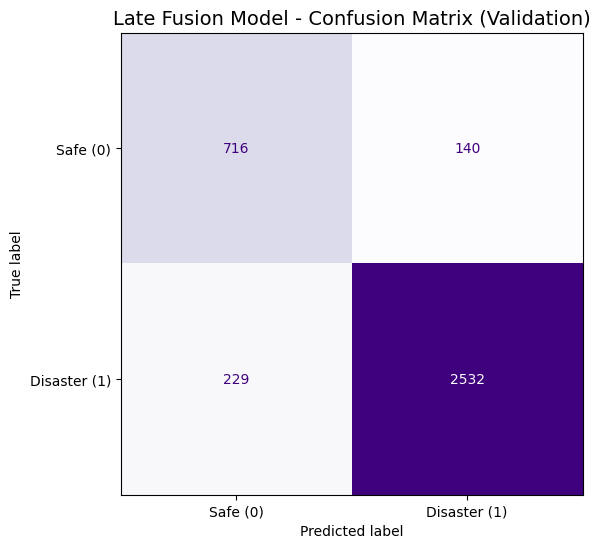
\includegraphics[width=0.9\linewidth]{nb03_img01.png}
        \caption{Confusion matrix on the validation set.}
        \label{fig:fusion_confmat_new}
    \end{subfigure}
    \begin{subfigure}{0.47\textwidth}
        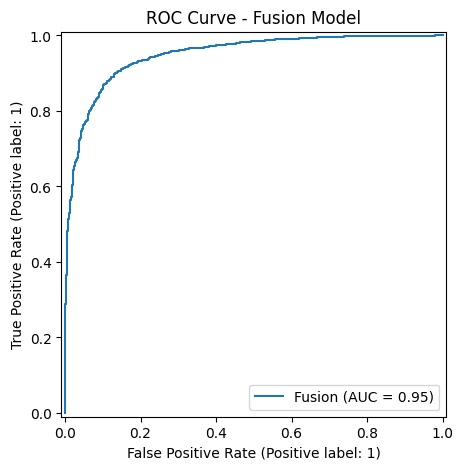
\includegraphics[width=0.9\linewidth]{nb03_img02.png}
        \caption{ROC curve on the validation set.}
        \label{fig:fusion_roc_new}
    \end{subfigure}
    \caption{Refined fusion model evaluation results. The best checkpoint at epoch 2 achieves $89.80\%$ accuracy, binary F1 of $0.9321$, macro F1 of $0.8636$, and ROC-AUC of $0.9491$.}
    \label{fig:fusion_eval_new}
\end{figure}

The fusion model shows the most striking improvement across the two runs. ROC-AUC increased from $0.8910$ to $0.9491$, and the number of false negatives—disaster tweets incorrectly classified as safe—dropped from $541$ to $229$, a $57.7\%$ reduction. This dramatic gain is largely attributable to the improved text encoder: because the fusion head trains on frozen text and vision embeddings, the quality of those embeddings sets an upper bound on fusion performance. The refined text branch, by selecting a checkpoint at epoch 3 rather than epoch 1, provides substantially more balanced text representations. The initial epoch-1 text encoder was biased toward predicting disaster (high recall, low precision on the safe class), which propagated into the fusion head and inflated the safe-class false negative rate. The epoch-3 encoder, having had more training epochs to adjust its internal representations under the weighted loss, provides richer and more discriminative embeddings that the fusion MLP can exploit more effectively.

The training curve for the fusion head also reveals an important characteristic of frozen-encoder late fusion: training loss decreases smoothly and monotonically, while validation loss and accuracy oscillate after the first two epochs. This pattern arises because the frozen encoders provide fixed-dimensional representations that the small MLP head can fit rapidly—after epoch 2 the head begins to overfit the particular co-occurrence patterns in the training split that do not generalize to the validation set. The F1-macro early stopping criterion correctly identifies epoch 2 as the point of best generalization.

\subsection{Quantitative Comparison}
Table~\ref{tab:model_comparison_full} presents the complete quantitative comparison across all three model variants and both training runs. Initial accuracy values for the vision and fusion branches are computed from the confusion matrix values reported in the initial run; initial macro F1 was not tracked separately for these branches.

\begin{table}[H]
\centering
\caption{Validation performance comparison: initial vs refined training runs across all model variants. Initial vision/fusion accuracy derived from reported confusion matrices; initial macro F1 not separately reported for those branches.}
\label{tab:model_comparison_full}
\begin{tabular}{@{}llccc@{}}
\toprule
\textbf{Model} & \textbf{Run} & \textbf{Val Accuracy} & \textbf{Val Macro F1} & \textbf{Val ROC-AUC} \\ \midrule
\multirow{2}{*}{Text-only DistilBERT}   & Initial & 81.94\% & ---    & 0.8654 \\
                                         & Refined & 80.01\% & 0.7997 & 0.8749 \\ \midrule
\multirow{2}{*}{Vision-only ResNet50}   & Initial & 82.37\% & 0.8237 & 0.9040 \\
                                         & Refined & 83.02\% & 0.8302 & 0.9059 \\ \midrule
\multirow{2}{*}{Late Fusion (Text + Image)} & Initial & 80.71\% & 0.7658 & 0.8910 \\
                                             & Refined & 89.80\% & 0.8636 & 0.9491 \\ \bottomrule
\end{tabular}
\end{table}

\subsection{Discussion}
The results demonstrate two complementary findings. First, the F1-macro early stopping and cosine warmup together produced a more balanced text encoder: although raw accuracy decreased by $1.93$ percentage points, macro F1 improved and ROC-AUC increased from $0.8654$ to $0.8749$, reflecting a shift away from majority-class hedging and toward genuine minority-class recovery. For the vision branch, the changes produced modest gains consistent with a principled checkpoint selection replacing a less discriminating loss-based criterion.

Second, and more significantly, the fusion model benefited disproportionately from the improved text branch. A $9.78$ percentage point increase in macro F1 (from $0.7658$ to $0.8636$) and a $5.81$ percentage point increase in ROC-AUC (from $0.8910$ to $0.9491$) substantially surpass what either unimodal branch achieved individually. The false negative count falling from $541$ to $229$ highlights the practical consequence: the refined fusion model misses $312$ fewer real disaster tweets on the validation set. This is consistent with the OR-label task design, in which disaster-related evidence can appear in either the text or the image channel, and the fusion head's ability to recover such cases depends critically on the quality of both encoders.

The largest multimodal gain is concentrated in F1 rather than raw accuracy. This is the expected pattern under class imbalance: accuracy measures aggregate correctness, which can be inflated by strong majority-class performance, while F1 and ROC-AUC directly capture the ability to discriminate between classes. The fact that all three refined models improve on ROC-AUC confirms that the improvements reflect genuine gains in discriminative power rather than artifacts of threshold tuning.


% ==========================================
\section{System Implementation and UI}
% ==========================================
\subsection{User Interface (GUI)}
We implemented a Streamlit chatbot-style interface in \texttt{app/streamlit\_app.py}. The UI uses a chat-style layout: users may submit tweet text, attach an image (\texttt{jpg/jpeg/png}), or provide both; at least one of text or image must be present. The model returns the predicted label (\textit{disaster} or \textit{not\_disaster}) together with a confidence score. Built-in example buttons demonstrate model behavior on a clearly non-informative tweet and a realistic disaster-style report.

The inference service (\texttt{inference/service.py}) applies the same \texttt{clean\_tweet()} preprocessing used during training, tokenizes the text, transforms the image using evaluation transforms (or substitutes a blank black image if none is provided), and passes both through the full fusion model to return softmax class probabilities.

Figures~\ref{fig:streamlit_text}--\ref{fig:streamlit_multi} show screenshots from our deployment for \textbf{text-only}, \textbf{image-only}, and \textbf{text plus image} inputs. Without an uploaded photo, the vision path receives a placeholder image at inference.

\begin{figure}[H]
    \centering
    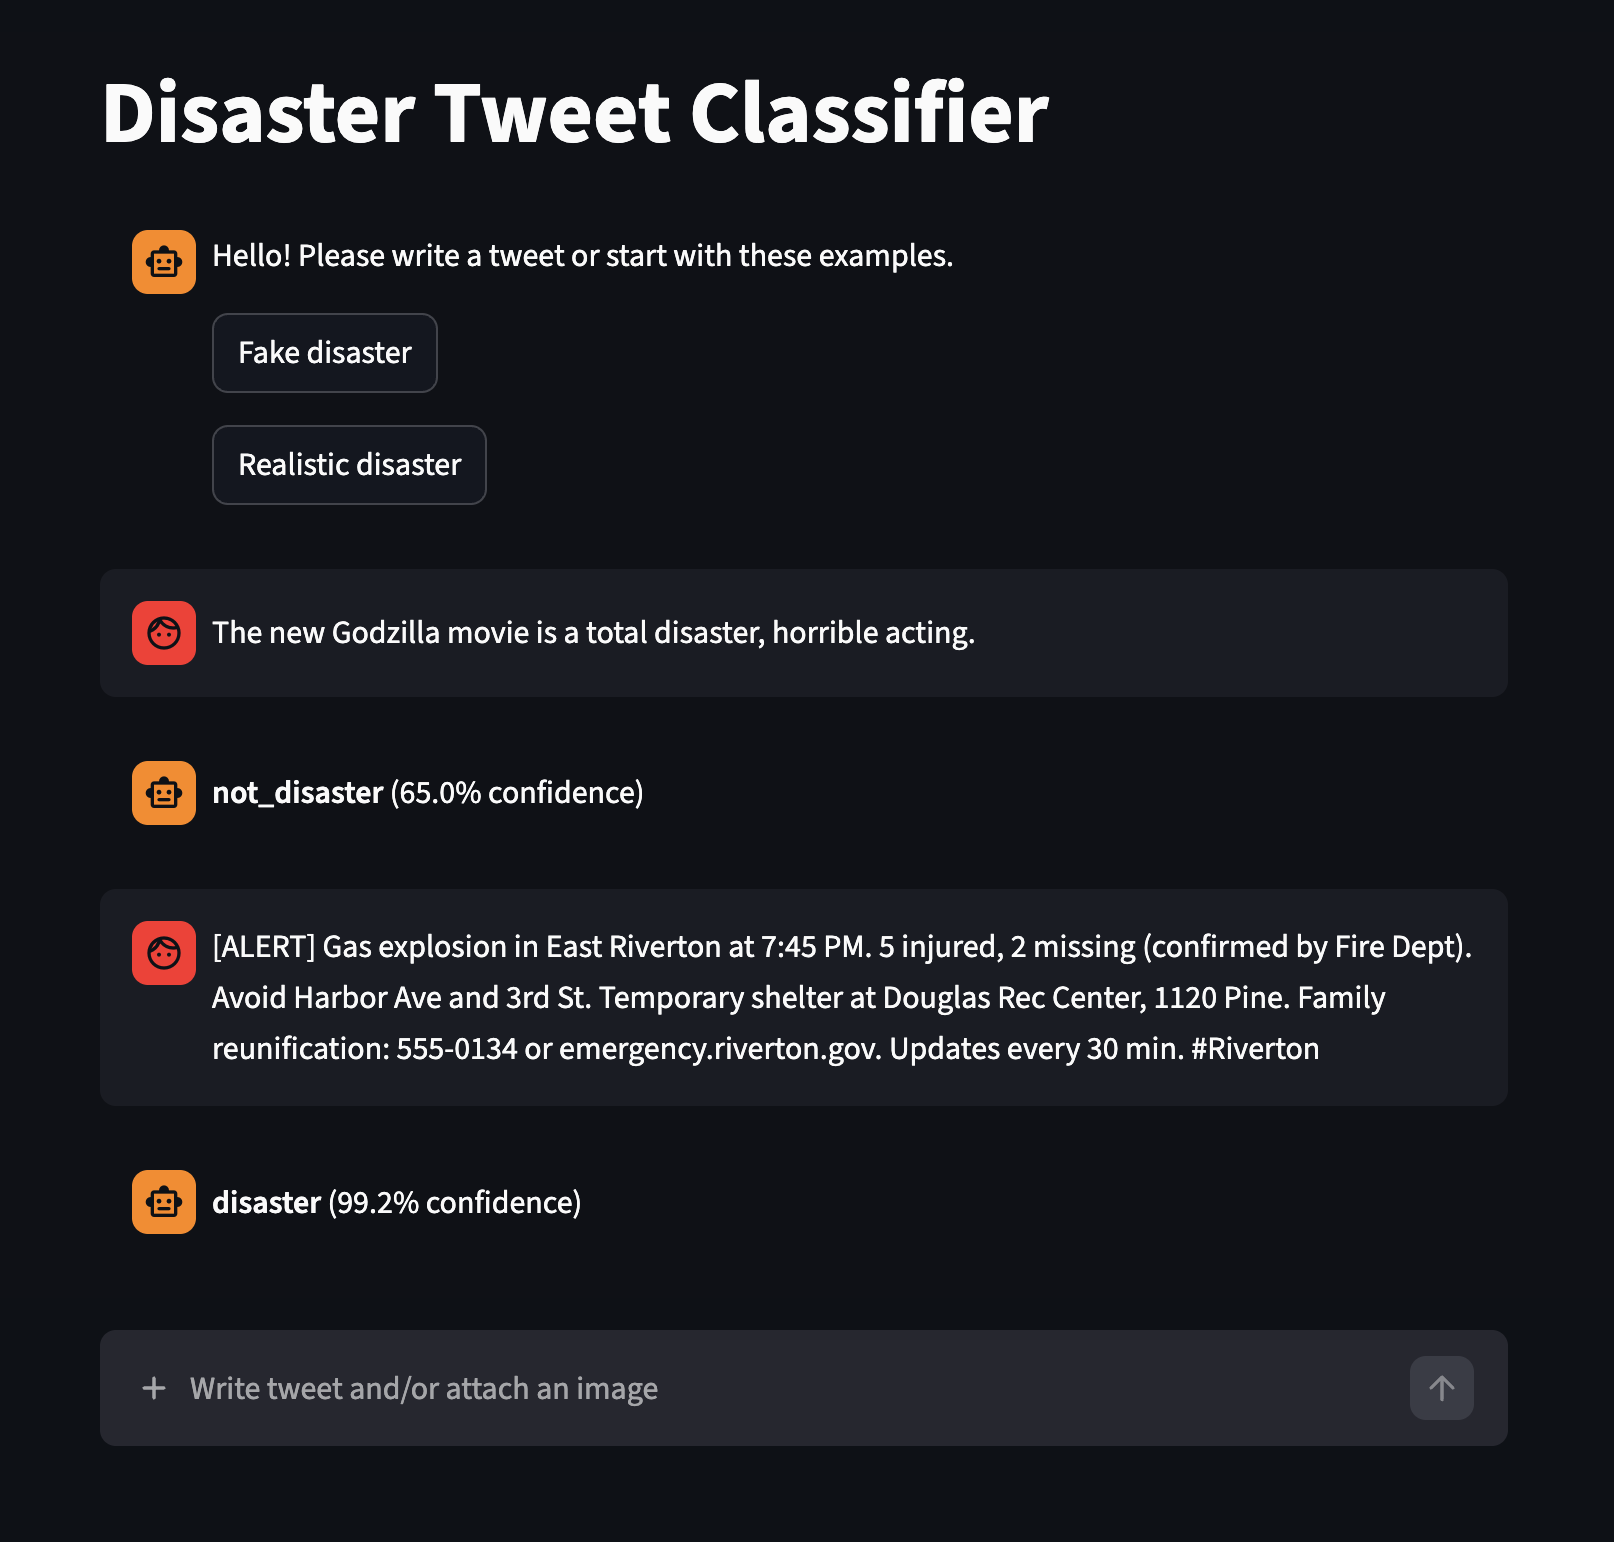
\includegraphics[width=0.92\linewidth]{streamlit_text.png}
    \caption{Streamlit UI: \textbf{text-only} sessions.}
    \label{fig:streamlit_text}
\end{figure}

\begin{figure}[H]
    \centering
    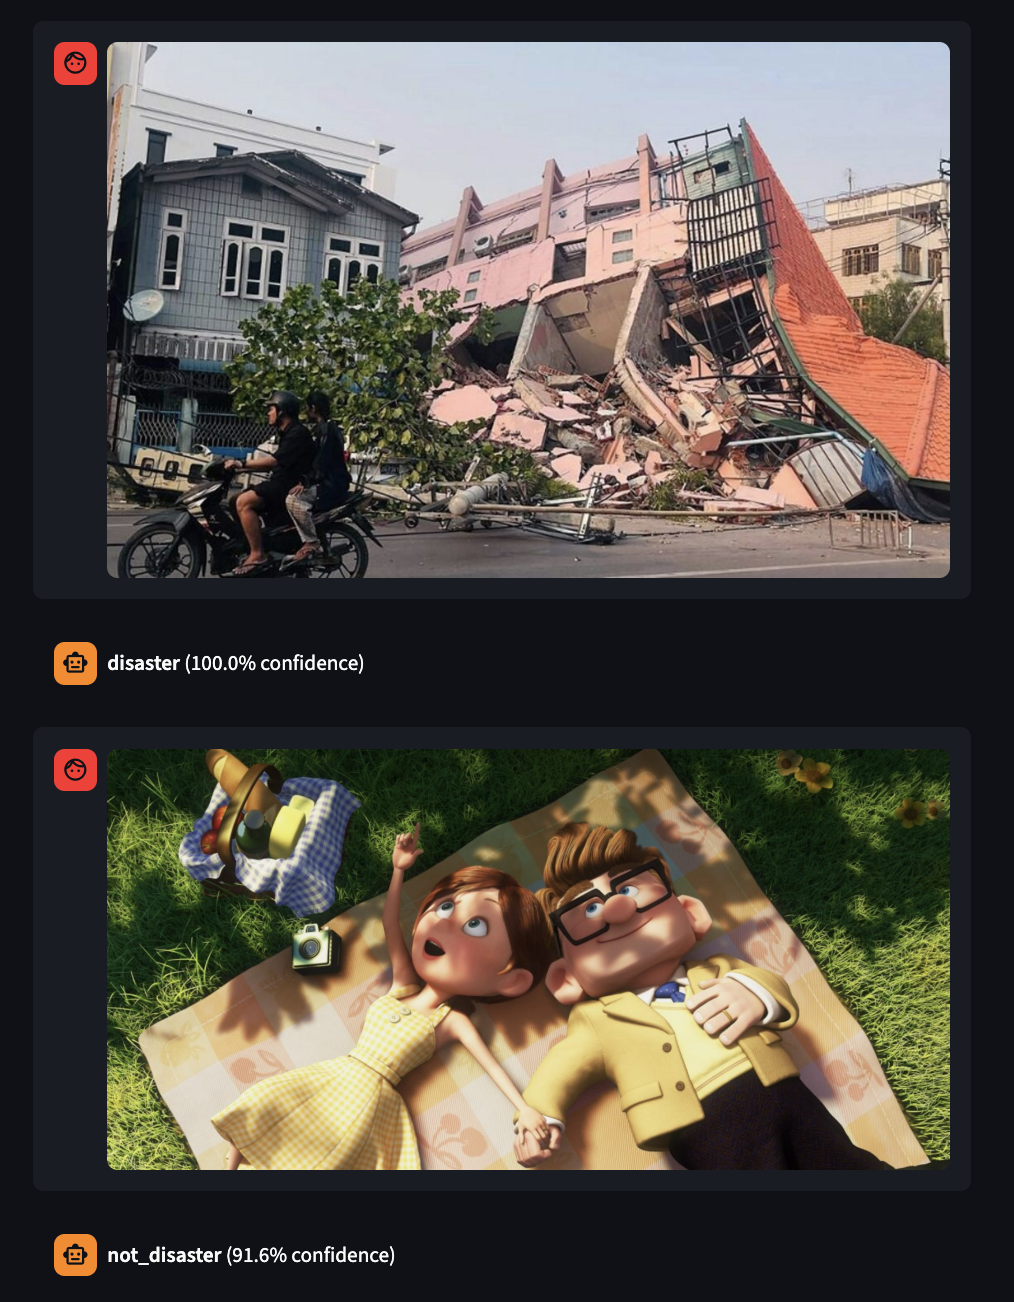
\includegraphics[width=0.92\linewidth]{streamlit_img.png}
    \caption{Streamlit UI: \textbf{image-only} sessions.}
    \label{fig:streamlit_img}
\end{figure}

\begin{figure}[H]
    \centering
    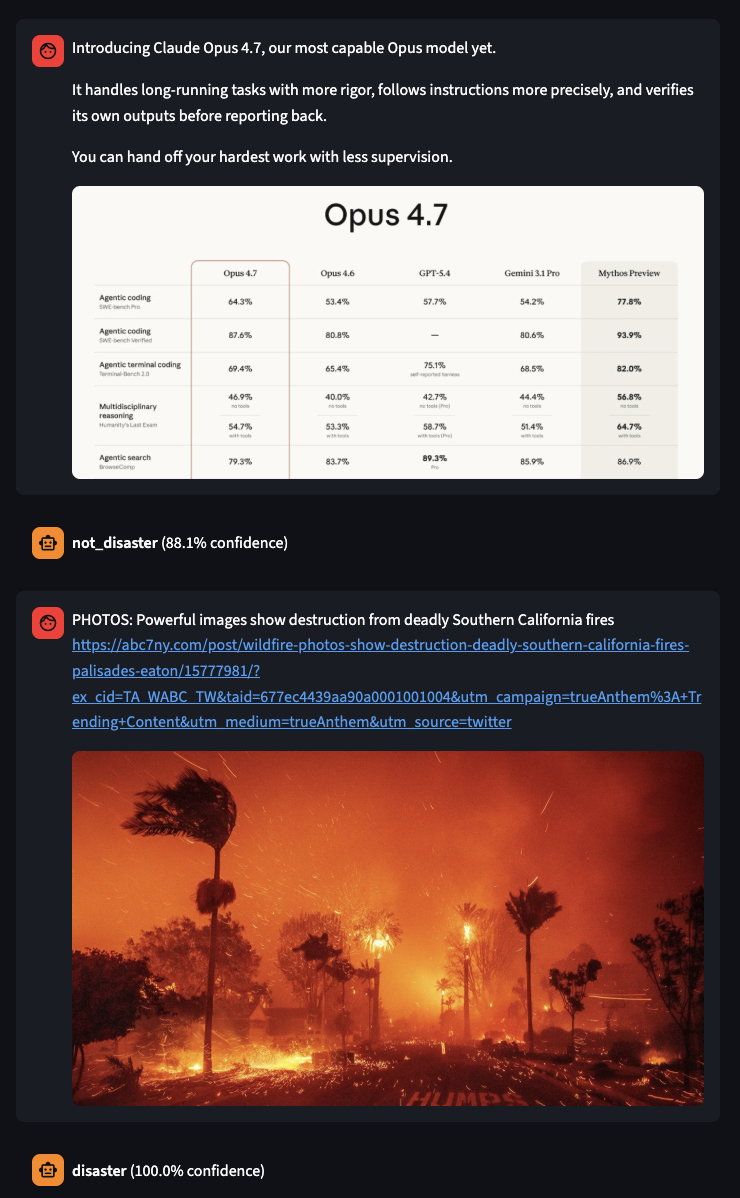
\includegraphics[width=0.80\linewidth]{streamlit_multi.png}
    \caption{Streamlit UI: \textbf{multimodal} sessions (tweet text with image).}
    \label{fig:streamlit_multi}
\end{figure}

\subsection{Reproducibility and Codebase}
Dependencies are listed in \texttt{requirements.txt}. Install with \texttt{pip install -r requirements.txt}.

\subsubsection*{Training from Scratch}
Run the following notebooks in order on Google Colab (GPU recommended). Mount Google Drive before starting; checkpoints are saved directly to \texttt{/content/drive/MyDrive/checkpoints/} during training and do not require a separate save step.
\begin{enumerate}
    \item \textbf{\texttt{00\_dataloader.ipynb}} --- Download Kaggle \texttt{train.csv} and \texttt{CrisisMMD\_v2.0} via \texttt{gdown} and verify paths.
    \item \textbf{\texttt{01\_text\_branch\_train.ipynb}} --- Fine-tune DistilBERT on the combined Kaggle + CrisisMMD text pool. Saves \texttt{checkpoints/text\_branch/} (Hugging Face format: \texttt{config.json}, \texttt{model.safetensors}, tokenizer files).
    \item \textbf{\texttt{02\_vision\_branch\_train.ipynb}} --- Fine-tune ResNet50 on CrisisMMD images.\\Saves \texttt{checkpoints/vision\_brain.pth}.
    \item \textbf{\texttt{03\_fusion\_layer\_train.ipynb}} --- Train the MLP fusion head with frozen text and vision encoders. Requires the checkpoints from steps 2 and 3. Saves \texttt{checkpoints/fusion\_brain.pth}.
\end{enumerate}

\subsubsection*{Reproducing Metrics and Visualizations Without Retraining}
If checkpoints already exist on Google Drive, all evaluation metrics and plots (confusion matrix, ROC curve) can be reproduced without re-running training:
\begin{enumerate}
    \item Mount Google Drive in Colab. The Drive path \texttt{/content/drive/MyDrive/checkpoints/} is configured at the top of each notebook.
    \item Open the target notebook.
    \item Run the setup cells (Drive mount, imports, path definitions).
    \item Skip to the \textbf{``Evaluation on best checkpoint''} section and run those cells. Each notebook loads the saved weights, calls \texttt{evaluate()}, and produces the confusion matrix and ROC curve.
\end{enumerate}

\subsubsection*{Running the Streamlit Frontend}
Copy the three checkpoint artifacts from Drive to a \texttt{checkpoints/} directory at the project root:
\begin{itemize}
    \item \texttt{checkpoints/text\_branch/} --- DistilBERT model directory
    \item \texttt{checkpoints/vision\_brain.pth} --- ResNet50 state dict
    \item \texttt{checkpoints/fusion\_brain.pth} --- Fusion MLP state dict
\end{itemize}
Then launch the app:
\begin{verbatim}
streamlit run app/streamlit_app.py
\end{verbatim}

% ==========================================
\section{Conclusion}
% ==========================================
This project demonstrates that a multimodal approach is effective for disaster-informative tweet classification. While text-only and vision-only models each provide strong individual signals, late fusion is expected to yield the best F1, indicating superior balance between precision and recall on imbalanced data. This supports our main hypothesis that text and image provide complementary evidence in noisy crisis settings.

The training pipeline was iteratively refined through direct observation of training curves. Early vision branch runs exhibited overfitting, addressed through differential learning rates, StepLR scheduling, and data augmentation. A shared \texttt{text\_cleaner.py} module ensures consistent preprocessing across training and inference, and \texttt{seed\_everything(42)} makes all runs reproducible across sessions.

For future work, we plan to (i) evaluate on event-held-out splits for stronger domain-shift robustness, (ii) improve calibration and threshold tuning for emergency triage, and (iii) experiment with partial encoder unfreezing and stronger augmentation strategies for additional multimodal gains. The CrisisMMD dataset also contains confidence scores that could be used to guide the model.

% --- References ---
\bibliographystyle{ieeetr}
\bibliography{refs}

\end{document}
